\chapter{Introduction}\index{Introduction}

\section{What is Sage?}

Algorithms in this Notes are implemented in Python programming language using SageMath (\url{https://www.sagemath.org}).


\begin{dBox}
SageMath is a free open-source mathematics software system licensed under the GPL.
It builds on top of many existing open-source packages: NumPy, SciPy, matplotlib, Sympy, Maxima, GAP, FLINT,
R and many more.
\end{dBox}

You can download binaries at \url{http://www.sagemath.org/download.html} for Mac, and Windows.

Note: Binaries for Windows are avaliable up to version 9.3 (late 2021).
For newer versions you will need to install it in WSL. Follow the instructions at\url{https://doc.sagemath.org/html/en/installation/index.html}.


There is also a cloud version available at https://cocalc.com/

% Using `sage -n jupyter` or running `SageMath 9.x Notebook` application (on Windows) you start jupyter notebook server on localhost:8888.

\noindent Documentation can be found at \url{https://doc.sagemath.org/html/en/index.html}.

\noindent We will moslty use \emph{graph theory} package \url{https://doc.sagemath.org/html/en/reference/graphs/index.html}

\section{Some examples of Sage Graph Theory objects and methods}

For representing undirected graphs we use the \texttt{Graph} class, while for representing directed graphs we use the \texttt{DiGraph} class.

\subsection{Undirected graphs}

Undirected graph is represented using \texttt{Graph} class.

\begin{sageCell}
    G = Graph({0:[1,2,3], 4:[0,2], 6:[1,2,3,4,5]})
\end{sageCell}
There are many methods to access the graph properties. For example, to get a list of vertices use \texttt{vertices} method.
\begin{sageCell}
    G.vertices()
\end{sageCell}
\begin{outCell}
    [0,1,2,3,4,5,6]
\end{outCell}


To display the graph, simply execute a cell with the graph variable name.
\begin{sageCell}
    G
\end{sageCell}

The output is a graphical representation of the graph. If we do not specify vertex coordinates (see below), Sage will use a spring embedder layout algorithm to compute the coordinates.
\begin{outImage}
    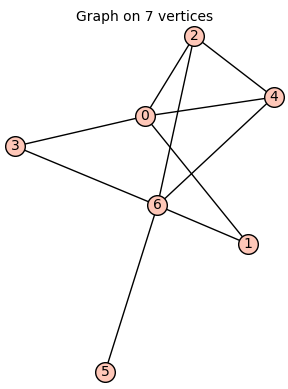
\includegraphics[width=6cm]{Images/Introduction/output_96_0.png}
\end{outImage}

If a graph is too large, it will not be displayed. In this case, or if you need to specify other display options, you can use the \texttt{plot} method. There are many options for the \texttt{plot} method, see \url{https://doc.sagemath.org/html/en/reference/plotting/sage/graphs/graph_plot.html} for details.

\medskip
For example. we can specify vertex colors using a dictionary, where keys are colors and values are lists of vertices.
\begin{sageCell}
    G.plot(vertex_colors={'red':[1],'green':[0,4]})
\end{sageCell}
\begin{outImage}
    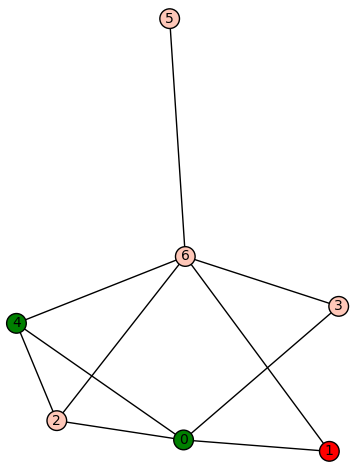
\includegraphics[width=6cm]{Images/Introduction/output_96_1.png}
\end{outImage}

\subsubsection{Some well-known graphs and graph families}

The famous Petersen graph.
\begin{sageCell}
    graphs.PetersenGraph()
\end{sageCell}
\begin{outImage}
    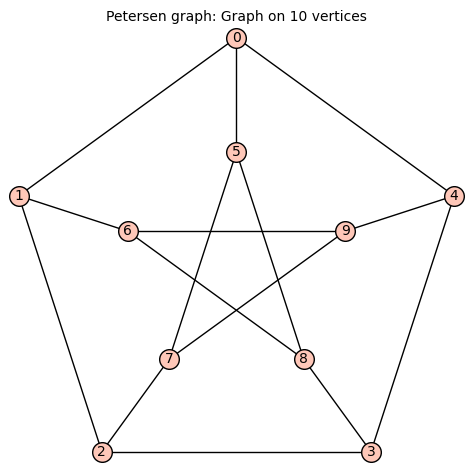
\includegraphics[width=8cm]{Images/Introduction/output_petersen.png}
\end{outImage}

Complete graphs $K_n$.
\begin{sageCell}
    graphs.CompleteGraph(7)
\end{sageCell}
\begin{outImage}
    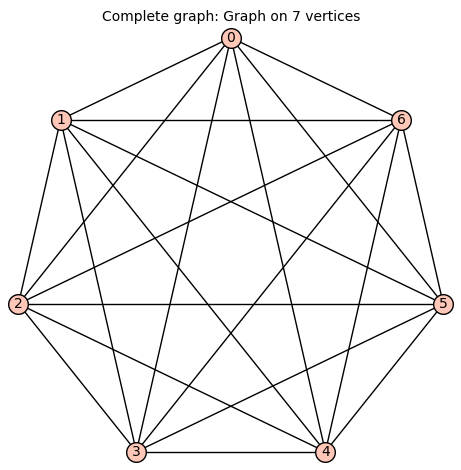
\includegraphics[width=8cm]{Images/Introduction/output_complete_7.png}
\end{outImage}

Cycle graphs $C_n$.
\begin{sageCell}
    graphs.CycleGraph(10)
\end{sageCell}
\begin{outImage}
    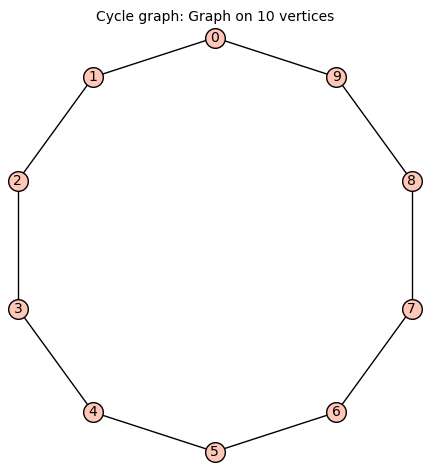
\includegraphics[width=8cm]{Images/Introduction/output_cycle_10.png}
\end{outImage}

Complete bipartite graphs $K_{n,m}$.
\begin{sageCell}
    graphs.CompleteBipartiteGraph(4, 10)
\end{sageCell}
\begin{outImage}
    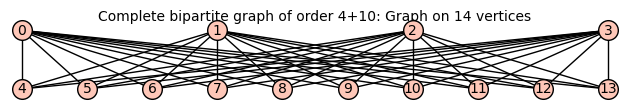
\includegraphics[width=0.8\linewidth]{Images/Introduction/output_complete_bipartite_4_10.png}
\end{outImage}

Grid graphs $G_{n,m}$.
\begin{sageCell}
    GG = graphs.GridGraph([4, 5])
    GG.plot()
\end{sageCell}
\begin{outImage}
    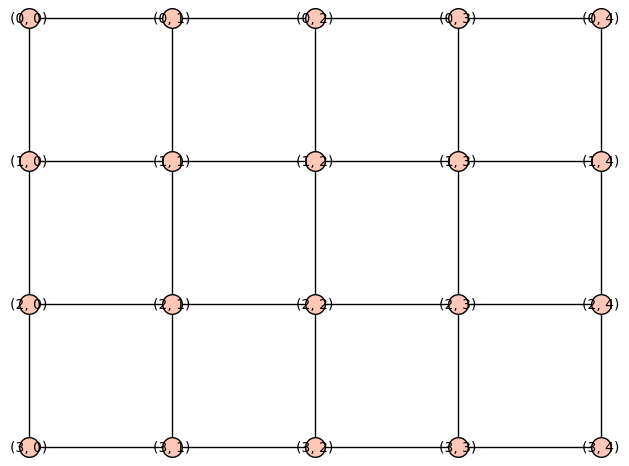
\includegraphics[width=0.8\linewidth]{Images/Introduction/output_grid_4_5.png}
\end{outImage}

\subsubsection{Randomly generated graphs}

Random graph on 10 nodes. Each edge is inserted independently with probability 0.3.
\begin{sageCell}
    graphs.RandomGNP(10, 0.3)
\end{sageCell}
\begin{outImage}
    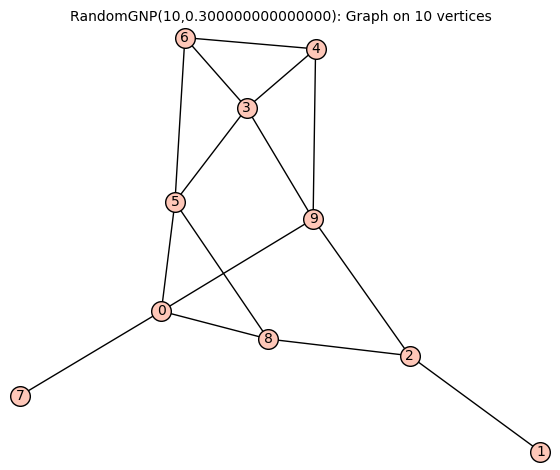
\includegraphics[width=0.8\linewidth]{Images/Introduction/output_random_10_03.png}
\end{outImage}

\subsubsection{Graph constructors}

From a list of edges.
\begin{sageCell}
    Graph([(1,2),(2,3),(3,1),(4,5)])
\end{sageCell}
\begin{outImage}
    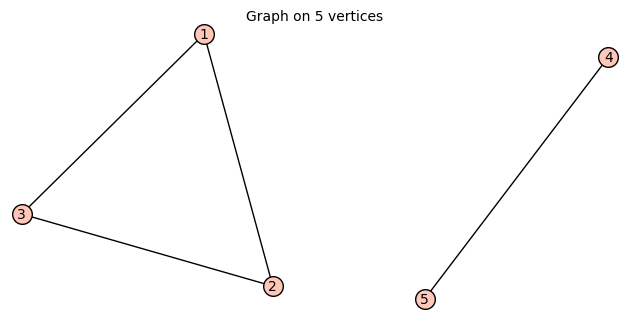
\includegraphics[width=10cm]{Images/Introduction/output_edge_list.png}
\end{outImage}

From an adjacency matrix.
\begin{sageCell}
    m = matrix([[int(i != j) for i in range(4)] for j in range(4)])
    m
\end{sageCell}
\begin{outCell}
    [0 1 1 1]
    [1 0 1 1]
    [1 1 0 1]
    [1 1 1 0]
\end{outCell}

\begin{sageCell}
    Graph(m)
\end{sageCell}
\begin{outImage}
    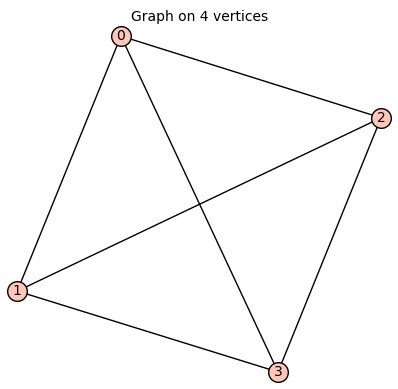
\includegraphics[width=6cm]{Images/Introduction/output_adjacency_matrix.png}
\end{outImage}

Graph to adjacency matrix.
\begin{sageCell}
    M = G.adjacency_matrix()
    m
\end{sageCell}
\begin{outCell}
    [0 1 1 1 1 0 0]
    [1 0 0 0 0 0 1]
    [1 0 0 0 1 0 1]
    [1 0 0 0 0 0 1]
    [1 0 1 0 0 0 1]
    [0 0 0 0 0 0 1]
    [0 1 1 1 1 1 0]
\end{outCell}

From/to graph6 format (compressed string representation of a graph).
\begin{sageCell}
    G = Graph('IheA@GUAo')
    G.plot()
\end{sageCell}
\begin{outImage}
    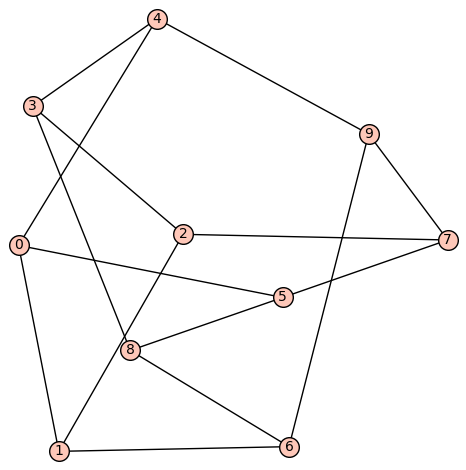
\includegraphics[width=6cm]{Images/Introduction/output_graph6.png}
\end{outImage}
\begin{sageCell}
    G.graph6_string()
\end{sageCell}
\begin{outCell}
    'IheA@GUAo'
\end{outCell}

Query a graph from local database
\url{http://doc.sagemath.org/html/en/reference/graphs/sage/graphs/graph_database.html}.
For example to get a list of all graphs on 7 vertices with diameter 5.
\begin{sageCell}
    Q = GraphQuery(display_cols=['graph6'], num_vertices=7, diameter=5)
    Q.show()
\end{sageCell}
\begin{outCell}
    Graph6
    --------------------
    F?`po
    F?gqg
    F@?]O
    F@OKg
    F@R@o
    FA_pW
    FEOhW
    FGC{o
    FIAHo
\end{outCell}

\subsection{Basic graph manipulation}

\begin{sageCell}
    G = Graph({0:[1,2,3], 4:[0,2], 6:[1,2,3,4,5]});
\end{sageCell}

\subsubsection{Access edges, verices, neighbors, etc.}

Access edges.
\begin{sageCell}
    G.edges(labels=False)
\end{sageCell}
\begin{outCell}
    [(0,1),(0,2),(0,3),(0,4),(1,6),(2,4),(2,6),(3,6),(4,6),(5,6)]
\end{outCell}
Note: Edges can have labels. To get a list of edges without labels, use \texttt{labels=False} option. Without this option we get
\begin{outCell}
    [(0,1,None),(0,2,None),(0,3,None),(0,4,None),(1,6,None),(2,4,None),
    (2,6,None),(3,6,None),(4,6,None),(5,6,None)]
\end{outCell}

To check if there is an edge between two vertices use
\begin{sageCell}
    G.has_edge(1,2)
\end{sageCell}
\begin{outCell}
    False
\end{outCell}

Access vertices.
\begin{sageCell}
    G.vertices()
\end{sageCell}
\begin{outCell}
    [0,1,2,3,4,5,6]
\end{outCell}

Access neighbors of a vertex.
\begin{sageCell}
    G.neighbors(0)
\end{sageCell}
\begin{outCell}
    [1,2,3,4]
\end{outCell}

Degree of a vertex is a number of its neighbors
\begin{sageCell}
    G.degree(0)
\end{sageCell}
\begin{outCell}
    4
\end{outCell}

To list degrees of all vertices use
\begin{sageCell}
    G.degree()
\end{sageCell}
\begin{outCell}
    [4,3,3,2,3,2,5]
\end{outCell}

Access number of vertices, edges
\begin{sageCell}
    [G.num_verts(),G.num_edges()]
\end{sageCell}
\begin{outCell}
    [7,10]
\end{outCell}

Vertices of a graph can be any hashable objects, not just integers. For example:
\begin{sageCell}
    X=Graph({'A':[1,2],'B':[(1,2),5,'A']})
    X.plot()
\end{sageCell}
\begin{outImage}
    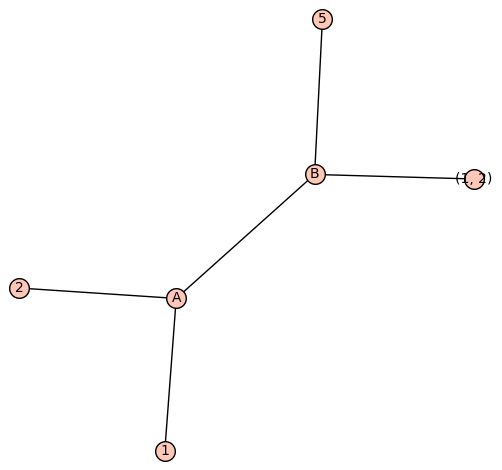
\includegraphics[width=8cm]{Images/Introduction/output_hashable.png}
\end{outImage}

\subsubsection{Add/remove vertices, edges}

Add a vertex.
\begin{sageCell}
    G.add_vertex('a')
\end{sageCell}

Method \verb|add_vertex| without arguments adds a single vertex with the smallest available label.
\begin{sageCell}
    newv = G.add_vertex()
    newv
\end{sageCell}
\begin{outCell}
    7
\end{outCell}

\begin{sageCell}
    G.vertices(sort=False)
\end{sageCell}
\begin{outCell}
    ['a',7,0,1,2,3,4,5,6]
\end{outCell}



